% -*- latex -*-

\documentclass[conference]{IEEEtran}

\usepackage{amsfonts}
\usepackage{amssymb}
\usepackage[cmex10]{amsmath}
\usepackage{booktabs}
%\usepackage{enumitem}
\usepackage{graphicx}
\usepackage{fancyvrb}
\usepackage{ifthen}
\usepackage{cite}
\usepackage[caption=false,font=footnotesize]{subfig}
\usepackage{tabulary}
\usepackage{url}
\usepackage{xspace}
\usepackage[pdfborder={0 0 0}]{hyperref}
\usepackage{verbatim}

\usepackage{color}
\definecolor{yellow}{rgb}{1,1,0}
\definecolor{black}{rgb}{0,0,0}
\definecolor{ltcyan}{rgb}{.75,1,1}
\definecolor{red}{rgb}{1,0,0}
\definecolor{gray}{rgb}{.6,.6,.6}
\definecolor{darkred}{rgb}{0.5,0,0}
\definecolor{darkgreen}{rgb}{0,0.5,0}

% Cite commands I use to abstract away the different ways to reference an
% entry in the bibliography (superscripts, numbers, dates, or author
% abbreviations).  \scite is a short cite that is used immediately after
% when the authors are mentioned.  \lcite is a full citation that is used
% anywhere.  Both should be used right next to the text being cited without
% any spacing.
\newcommand*{\lcite}[1]{~\cite{#1}}
\newcommand*{\scite}[1]{~\cite{#1}}

\newcommand{\etal}{et al.}

\newcommand*{\keyterm}[1]{\emph{#1}}

\newcommand{\fix}[1]{{\color{red}\textsc{[#1]}}}

% Avoid putting figures on their own page.
\renewcommand{\textfraction}{0.05}
\renewcommand{\topfraction}{0.95}
\renewcommand{\bottomfraction}{0.95}

% Make sure this is big enough so that only big figures end up on their own
% page but small enough so that if a figure does have to be on its own
% page, it won't push everything to the bottom because it's not big enough
% to have its own page.
\renewcommand{\floatpagefraction}{.75}

% Allows multiline equations (align environment) to break across pages.
\allowdisplaybreaks[4]

\newenvironment{packed_itemize}{
  \begin{itemize}[noitemsep]
}{
  \end{itemize}
}


\begin{document}

\sloppy

%
% paper title
% can use linebreaks \\ within to get better formatting as desired
\title{A Formal Metric for Large-Scale Parallel Algorithm Performance Analysis}


% author names and affiliations
% use a multiple column layout for up to three different
% affiliations
%% \author{\IEEEauthorblockN{Michael Shell}
%% \IEEEauthorblockA{School of Electrical and\\Computer Engineering\\
%% Georgia Institute of Technology\\
%% Atlanta, Georgia 30332--0250\\
%% Email: http://www.michaelshell.org/contact.html}
%% \and
%% \IEEEauthorblockN{Homer Simpson}
%% \IEEEauthorblockA{Twentieth Century Fox\\
%% Springfield, USA\\
%% Email: homer@thesimpsons.com}
%% \and
%% \IEEEauthorblockN{James Kirk\\ and Montgomery Scott}
%% \IEEEauthorblockA{Starfleet Academy\\
%% San Francisco, California 96678-2391\\
%% Telephone: (800) 555--1212\\
%% Fax: (888) 555--1212}}

\author{
  \IEEEauthorblockN{Kenneth Moreland}
  \IEEEauthorblockA{
    Sandia National Laboratories\\
    Email: kmorel@sandia.gov}
  \and
  \IEEEauthorblockN{Ron Oldfield}
  \IEEEauthorblockA{
    Sandia National Laboratories\\
    Email: raoldfi@sandia.gov}
}

% conference papers do not typically use \thanks and this command
% is locked out in conference mode. If really needed, such as for
% the acknowledgment of grants, issue a \IEEEoverridecommandlockouts
% after \documentclass

% for over three affiliations, or if they all won't fit within the width
% of the page, use this alternative format:
% 
%\author{\IEEEauthorblockN{Michael Shell\IEEEauthorrefmark{1},
%Homer Simpson\IEEEauthorrefmark{2},
%James Kirk\IEEEauthorrefmark{3}, 
%Montgomery Scott\IEEEauthorrefmark{3} and
%Eldon Tyrell\IEEEauthorrefmark{4}}
%\IEEEauthorblockA{\IEEEauthorrefmark{1}School of Electrical and Computer Engineering\\
%Georgia Institute of Technology,
%Atlanta, Georgia 30332--0250\\ Email: see http://www.michaelshell.org/contact.html}
%\IEEEauthorblockA{\IEEEauthorrefmark{2}Twentieth Century Fox, Springfield, USA\\
%Email: homer@thesimpsons.com}
%\IEEEauthorblockA{\IEEEauthorrefmark{3}Starfleet Academy, San Francisco, California 96678-2391\\
%Telephone: (800) 555--1212, Fax: (888) 555--1212}
%\IEEEauthorblockA{\IEEEauthorrefmark{4}Tyrell Inc., 123 Replicant Street, Los An3geles, California 90210--4321}}


\maketitle


\begin{abstract}
Performance measurement of parallel algorithms is well studied and well
understood. However, a flaw in our performance metrics is that they rely on
comparisons to serial performance with the same input. This comparison is
convenient for theoretic complexity analysis but impossible to perform in
large-scale empirical studies with data sizes far too large to run on a
single serial computer.  Consequently, scaling studies currently rely ad
hoc methods that, although effective, have no grounded mathematical models.
In this position paper we advocate using a rate-based model that has a
concrete meaning relative to speedup and efficiency and that can be used to
unify strong and weak scaling studies.
\end{abstract}

\section{Introduction}

\noindent
The theory of parallel performance is well studied and often used in
practice, yet all our current models are limited by their reliance on
serial behavior.

\subsection{Performance Analysis Theory}

\noindent
The \keyterm{speedup} of a parallel algorithm is defined as
\begin{equation}
  S(n,p) = \frac{T^*(n)}{T(n,p)}
  \label{eq:Speedup}
\end{equation}
where $T(n,p)$ is the time it takes to run the parallel algorithm on $p$
processing elements with an input of size $n$ and $T^*(n)$ the time for the
best serial algorithm on the same input. The best possible serial algorithm
may be different than the parallel algorithm although using the same
algorithm is also common practice.

In theory the best possible speedup achievable\lcite{Faber1986} is $S(n,p)
= p$ (although in practice superlinear measurements are possible). Thus, we
measure the \keyterm{efficiency} as the ratio of the observed speedup to
the ideal speedup.
\begin{equation}
  E(n,p) = \frac{S(n,p)}{p} = \frac{T^*(n)}{p \; T(n,p)}
  \label{eq:Efficiency}
\end{equation}

Amdahl\scite{Amdahl1967} famously observes the limits of scaling any
parallel algorithm based on the computation fraction $f$ that exists in any
algorithm that is inherently serial. The equation derived from this
observation is known as \keyterm{Amdahl's law}.
\begin{equation}
  S(n,p) \leq \frac{1}{f + (1-f)/p}
  \label{eq:Amdahl}
\end{equation}

Gustafson\scite{Gustafson1988} observes that the serial fraction tends to
go down for larger data sizes in parallel algorithms, which justifies the
use of parallel computing for large problems. The \keyterm{Gustafson-Barsis
  law} reformulates speedup in terms of the parallel execution rather than
the serial execution
\begin{equation}
  S(n,p) \leq p + f(1-p)
  \label{eq:GustafsonBarsis}
\end{equation}
This law shows that speedup can be increased indefinitely as
long as the serial fraction drops commensurately with the processing
element increase. Grama \etal\scite{Grama1993} introduce an
\keyterm{isoefficiency} metric that determines how much a problem needs to
grow to maintain linear speedup.

Performance analysis theory is reviewed in much more detail in many
parallel computing textbooks such as Quinn's\scite{Quinn2004}.

\subsection{Limitations of Performance Analysis}

\noindent
Although our definition for speedup and its derived quantities work well
for theoretical complexity analysis, they all rely in some way on knowing
the serial performance. With large-scale simulations today reaching orders
of billions to trillions of
elements\lcite{Bernaschi2013,Rossinelli2013,Bussmann2013,Habib2013},
directly measuring serial performance is impossible. The Gustafson-Barsis
law needs only the serial fraction, but estimates for serial
fraction such as the \keyterm{Karp-Flatt} metric\lcite{Karp1990} require
knowing the serial performance anyway.

Because of this issue, many studies attempt to assess scalability directly
from an algorithm's running time relative to the number of processing
elements, which is called \keyterm{strong scaling}\lcite{Kaminsky2014}.
Because a parallel algorithm with perfect speedup has a running time
proportional to $1/p$, we look for time behavior that follows a roughly
hyperbolic plot that asymptotically a number close to zero (representing
the overhead). However, all but the very worst scaling algorithms tend to
asymptotically approach some constant time, which makes it difficult to
distinguish when an algorithm is actually scaling well. Often we try to
rectify the problem by plotting the running time using log scaling for both
the number of processing elements and the time because perfect scaling on
this plot is a straight line. However, overheads of any polynomial order
are also straight lines, which again makes it difficult to differentiate
good and bad scaling.

Another common approach is to measure \keyterm{weak scaling}\lcite{Kaminsky2014}.
In weak scaling the size of the input data is increased with the number of
processing elements. Typically the input is kept proportional to the number
of processing elements. In this case a perfectly scaling algorithm will
have the same running time for all runs. Although an important
characteristic, weak scaling should also be coupled with strong scaling to
get a complete picture. Also, analyzing weak scaling this way requires the
ability to vary the data proportionally with the processing elements, which
is not always possible.  For example, some simulations might adaptively
remesh based on some criteria, which means the size of the data can be
modified but not directly set by an analyst.

Some studies use an ad hoc version of speedup that replaces the
immeasurable $T^*(n)$ with some arbitrarily chosen measurement, usually the
time run on the smallest number of processing elements. The problem with
this approach is that the absolute ``speedup'' values are meaningless and
any weak scaling comparisons are impossible.

Finally, some studies use rate in terms of the size of input computed per
unit time rather than absolute run time to assess
scalability\lcite{Kaminsky2014}. Rate is formally defined as
\begin{equation}
  R(n,p) = \frac{n}{T(n,p)}
  \label{eq:Rate}
\end{equation}
Some analysts have discovered that rate, being essentially a reciprocal of
time, provides a much better visual analysis of scaling, and it is
an essential the mechanism advocated in this position paper.

This paper will establish a realistic definition of speedup and efficiency
that can be easily measured empirically. Furthermore, we will demonstrate
how rate can be used as a proxy for speedup and can unify strong and weak
scaling to provide a more complete analysis.


\section{Deriving Efficiency from Cost Analysis}
\label{sec:CostAnalysis}

\noindent
In this section we will use \keyterm{cost}, a metric that is simple to
measure, to define efficiency in lieu of the immeasurable speedup. Cost is
intuitively the number of processing elements used multiplied by the amount
of time they are used.
\begin{equation}
  C(n,p) = p \; T(n,p)
  \label{eq:Cost}
\end{equation}
Cost is sometimes used in theoretical algorithm analysis\lcite{JaJa1992}
and is often used for HPC allocations, which are typically measured in
core-hours.

Clearly the most efficient algorithm will be the one that costs the least
to run. Although we expect the cost to go up with the problem size, a
perfectly scaled algorithm will cost the same regardless of how many
processors are used. That is, adding processors the reduces time. Given a
strong scaling study on a problem of a particular size, we can identify the
best (minimal) cost, $C^*(n)$ using $p^*$ processing elements. With this
best cost we can redefine efficiency as the ratio of this best cost to the
actual cost.
\begin{equation}
  E(n,p) = \frac{C^*(n)}{C(n,p)}
  \label{eq:EfficiencyCost}
\end{equation}

If we make the typical assumptions that the minimal cost is when the serial
algorithm is run ($C^*(n) = T^*(n)$), then we observe that
Equation~\ref{eq:EfficiencyCost} simplifies to
Equation~\ref{eq:Efficiency}, making this definition of efficiency
equivalent but broader than the traditional definition. And unlike the
traditional definition of efficiency, determining efficiency from cost is
straightforward at large scales.


\section{Strong and Weak Scaling with Cost Per Unit}
\label{sec:CostPerUnit}

\noindent
Our previous definition of efficiency (Equation~\ref{eq:EfficiencyCost})
works well for strong scaling where the data size is constant, but cannot
be compared across different data sizes for weak scaling. To describe
efficiency under weak scaling we define the new metric \keyterm{cost per
  unit}, $C_{/u}$. Cost per unit is the amortized computational cost for
one unit of data.
\begin{equation}
  C_{/u}(n,p) = \frac{C(n,p)}{n} = \frac{p \; T(n,p)}{n}
  \label{eq:CostPerUnit}
\end{equation}

The important feature of cost per unit is that under perfect scaling the
cost per unit is constant under any number of processing elements \emph{or}
data sizes. Thus, given multiple strong scaling studies over data of
different sizes, we can find the best (minimal) cost per unit $C_{/u}^*$
using $p^*$ processing elements and with data of size $n^*$. With this best
cost per unit we can adjusted to be comparable across all possible
configurations.
\begin{equation}
  E(n,p) = \frac{C_{/u}^*}{C_{/u}(n,p)}
  \label{eq:EfficiencyCostPerUnit}
\end{equation}

With this definition of efficiency we can combine strong and weak scaling
studies into one unified analysis. \fix{Does this need to be explained
  more?}


\begin{figure*}
  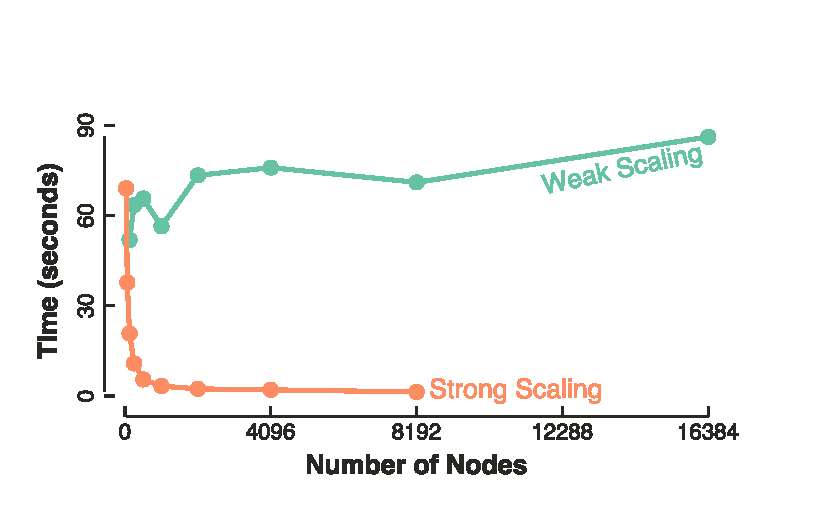
\includegraphics[width=.5\linewidth]{images/HabibTime}%
  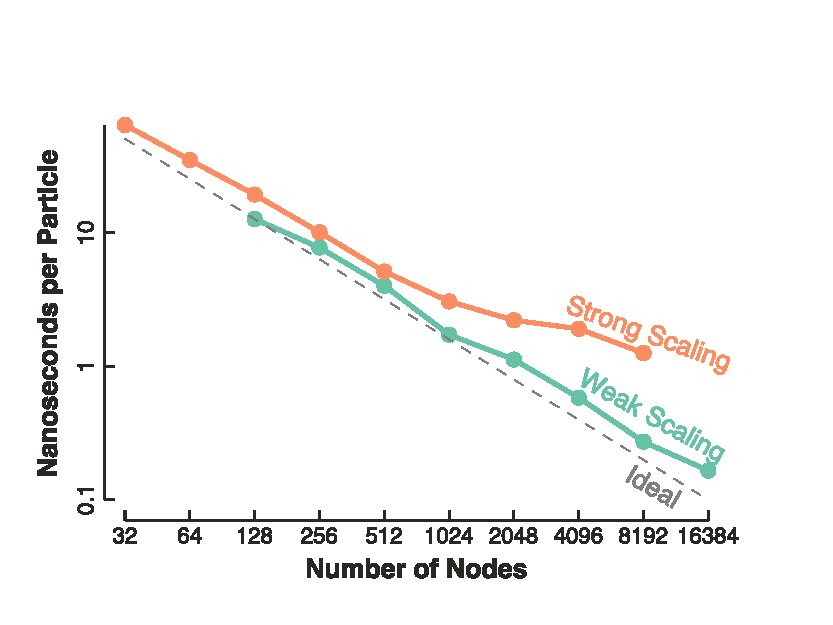
\includegraphics[width=.5\linewidth]{images/HabibTimePerParticle}
  \caption{Data from the Habib \etal\scite{Habib2013} Gordon Bell
    finalist. The left chart shows the data using a traditional time
    metric. The right chart replicates the presentation of Figure~3 in the
    original Habib \etal paper using an ad hoc metric and a log-log
    scale. Both charts present the data in a way to suggest near perfect
    scaling for both scaling studies.}
  \label{fig:HabibTraditional}
\end{figure*}

\begin{figure*}
  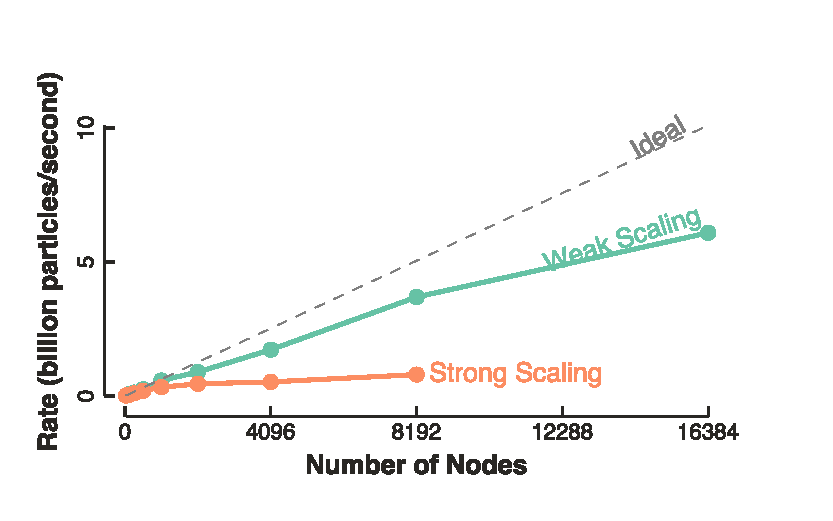
\includegraphics[width=.5\linewidth]{images/HabibRate}%
  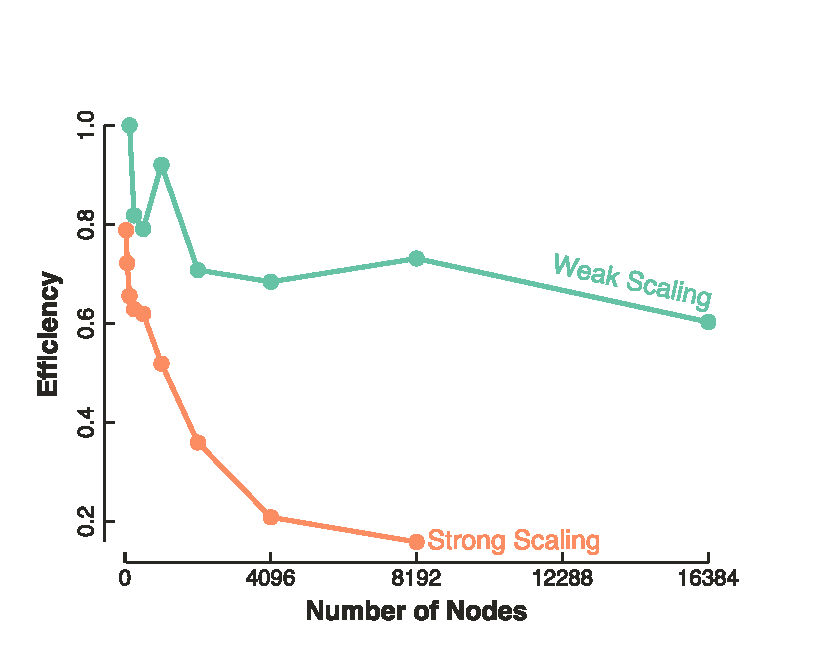
\includegraphics[width=.5\linewidth]{images/HabibEfficiency}
  \caption{Data from the Habib \etal\scite{Habib2013} Gordon Bell finalist
    using the rate (left) and efficiency (right) metrics advocated in this
    paper. These plots give a more realistic and visually measurable
    representation of scaling than the charts in
    Figure~\ref{fig:HabibTraditional}.}
  \label{fig:HabibBetter}
\end{figure*}


\section{Rate as a Proxy for Speedup}
\label{sec:RateProxy}

Both efficiency and speedup are good metrics for parallel performance
analysis. However, many analysts prefer using speedup, particularly for
visual (chart) analysis. This is because good scaling shows an upward
sloping speedup as jobs get larger whereas even a good scaling algorithm
will show a gradual drop-off from a perfect efficiency of 1.

Although there is no way to compute the speedup at large scales, we can
show that rate (Equation~\ref{eq:Rate}) is a valid proxy for speedup. If we
substitute rate for time in Equation~\ref{eq:Speedup}, we get the
following.
\begin{equation}
  S(n,p) = \frac{T^*(n)}{T(n,p)} = \frac{T^*(n)}{n} R(n,p)
  \label{eq:SpeedupFromRate}
\end{equation}

We can observe that for a given problem size (i.e. $n$ held constant) the
speedup is proportional to the rate. This means that the rate curve will
have the exact same shape as the speedup curve, and visually they will be
identical with the appropriate scaling of the ordinate axis.

For a proper parallel performance analysis we need to compare our measured
metrics with the ideal metrics. These ideal values are implicit in the
definition of efficiency ($E_\mathrm{ideal}(n,p) = 1$) and speedup
($S_\mathrm{ideal}(n,p) = p$). The ideal rate is dependent on the measured
best cost per unit and can be derived from
Equation~\ref{eq:EfficiencyCostPerUnit}.
\begingroup
\addtolength{\jot}{1ex} % Space equations a bit more. Fractions are cluttered.
\begin{align}
  \frac{C_{/u}^*}{C_{/u}(n,p)} &= E(n,p) \nonumber \\
  C_{/u}^* \frac{n}{p \; T(n,p)} &= E(n,p) \nonumber \\
  \frac{C_{/u}^*}{p} R(n,p) &= E(n,p) \nonumber \\
  \frac{C_{/u}^*}{p} R_\mathrm{ideal}(n,p) &= 1 \nonumber \\
  R_\mathrm{ideal}(n,p) &= p \frac{1}{C_{/u}^*}
\end{align}
\endgroup

Note that the curve for $R_\mathrm{ideal}(n,p)$ is independent of $n$,
which means we can use rate for both strong and weak scaling analysis.


\section{Example}

\noindent
In the previous sections we provided mathematical derivations to show how
to use rate as a proxy for speedup and to use cost per unit to find the
efficiency and ideal rate across all scales. In this section we demonstrate
using these metrics on real measured data.

\subsection{Gordon Bell Finalist}

\noindent
Our first data set comes a study by Habib \etal\scite{Habib2013}, which is
one of last year's Gordon Bell finalists. We choose this source because in
addition to showing impressive scaling, the authors make many measurements
across many scales and report the results completely enough to extract the
information and continue analysis. In particular, we look at the
performance data for scaling the full HACC code on Titan (Section~4.3.2 in
the original paper).

Figure~\ref{fig:HabibTraditional} shows the performance data from the
strong and weak scaling studies using a traditional time plot. The curves
for the data are very similar for what we would expect for perfect scaling:
a hyperbolic curve for strong scaling and a horizontal line for weak
scaling. Habib \etal also provide an ad hoc metric of time over data size
to unify the curve shape of the two plots, which is also replicated in
Figure~\ref{fig:HabibTraditional}. Again, both curves appear close to
perfect.

Figure~\ref{fig:HabibBetter} shows the same data using the rate and
efficiency metrics advocated in this paper. The weak scaling is shown to
scale off by a measurable fractions, which is to be expected when scaling
over 3 orders of magnitude. The strong scaling study is shown to diverge
very far from ideal.

Please note that it is not our intention to criticize the scaling shown by
Habib \etal\scite{Habib2013}. On the contrary, they show HACC to be world
class in scalability and demonstrate a consistent efficiency while scaling
the problem by an order of magnitude. Rather, our intention is to present
these data in a more informative and honest way. \fix{Could make a comment
  about being able to use a strong scaling study at a large data scale, but
  maybe that's not appropriate. Could reference that in the discussion
  instead.}

\subsection{Imperfect Scaling}

\noindent


\section{Discussion}

\noindent
Final recommendations? No log-log? Many short strong scale studies over
multiple scales?

Future work incorporating power in cost\lcite{Cameron2012}?


% use section* for acknowledgement
\section*{Acknowledgment}

\noindent
Sandia National Laboratories is a multi-program laboratory managed and
operated by Sandia Corporation, a wholly owned subsidiary of Lockheed
Martin Corporation, for the U.S. Department of Energy's National Nuclear
Security Administration under contract DE-AC04-94AL85000.

\bibliographystyle{IEEETranS}
\bibliography{FormalScalingMetric}

\end{document}


